\documentclass[12pt, a4paper]{report}
\usepackage[utf8]{inputenc}
\usepackage[left=40mm, right=20mm, top=30mm, bottom=30mm]{geometry}
\usepackage{titlesec}
\usepackage{xparse}
\usepackage{microtype}
\usepackage{graphicx}
\usepackage{amsmath}
\usepackage{placeins}
\usepackage{tikz}
\usetikzlibrary{shapes.geometric}

\titleformat{\chapter}[hang]{\Huge\bfseries}{\thechapter}{20pt}{\Huge\bfseries}

\graphicspath{{figures/}}

\NewDocumentCommand{\codeword}{v}{%
\texttt{{#1}}%
}


\title{Designing and implementing a tensor calculus}
\author{Farin Lippmann}
\date{August 2022}

% Area: Generic optimization
% Topic: Derivatives of higher-order tensor expressions
% Research Question: Can we design and implement an Einstein-notation-based tensor calculus for automatic symbolic differentiation of tensor expressions?

% Related Research: 
% - Matrix Calculus paper (uses ricci notation)
% - Tensor Calculus paper (basis for this thesis)
% - Algebra systems build scalar-valued functions for each tensor entry, inefficient [from Matrix Calculus Paper]

% Questions:
% - What am I improving over Matrix Calculus? 
%   -> Einstein notation instead of Ricci
%   -> Actually works on arbitrary tensor inputs
%   -> Cleanup inbetween derivation steps?
% - Why Einstein over Ricci?
%   -> Ricci is more complex, allows differentiating between tensors and their dual (multilinear maps)
%      which we don't need, tensors are strictly datastructures for us
%   -> Because we don't need the complexities of Ricci, Einstein allows a more elegant internal representation


\begin{document}
\maketitle

\chapter{Abstract}
\pagenumbering{gobble}

\chapter{Table of contents}
\pagenumbering{arabic}
\setcounter{page}{3}

\chapter{Introduction}

With the rise of machine learning applications, interest in optimization problems has been growing.
In these kinds of problems, one seeks to find values for a number of parameters that maximize or minimize a given scalar objective function.
While some optimization problems have a closed-form solution which can be computed directly, many can only be solved approximately.
When computing these approximate solutions, derivatives play a crucial role.
In particular, the first derivatives of the objective function are used in the ubiquitous gradient descent procedure.
In most optimization problems, multiple parameters need to be optimized simultaneously.
This means that derivatives need to be computed with respect to multiple variables, organized either in vectors, matrices or higher-order tensors.
Commonly used machine learning frameworks (like Tensorflow, PyTorch, Theano) focus heavily on the first derivatives of the objective function.

Higher-order derivatives can, however, also be of interest.
As an example, the matrix of second-order partial derivatives, called the Hessian, is used in the application of Newton's method, which can be more efficient than gradient descent for some problems.
Convexity checks constitute another application of higher-order derivatives.
The convexity of objective functions and their associated optimization problems play a major role in the field of optimization.
If a problem is strictly convex or concave, then it has a unique global optimum and the gradient descent algorithm can approximate it arbitrarily well.
To check for convexity, the objective function's Hessian matrix, the matrix of second-order partial derivatives, needs to be computed and checked for semidefiniteness.
If the function's inputs are naturally organized in a matrix or higher-order tensor, then the resulting Hessian will also be a higher-order tensor.
The prevalent machine learning frameworks have no way to directly compute these derivatives, and classical computer algebra systems struggle with efficiency, as they work on the level of individual tensor entries.

To bridge this gap, we design and implement a tensor calculus that allows for automatic symbolic differentiation of tensor expressions of any order.
Additionally, this calculus will use an Einstein-like notation to represent tensor products, rather than the more complex notation used in Ricci calculus.

This thesis builds on the work by Laue, Mitterreiter and Giesen, who have built a similar calculus for matrix derivatives [Matrix Calculus] and developed the theoretical foundation for an Einstein notation based tensor calculus [Tensor Paper].

The structure of the thesis is as follows.
First, the syntax of the calculus is developed in form of a grammar.
Then, the parsing and representation of tensor expressions are discussed, followed by a chapter on the differentiation process.

\chapter{A Syntax for Tensor Expressions}
\section{Aims}
In this chapter we develop the language that will be used to specify tensor expressions for differentiation.
To differentiate a tensor expression, three pieces of information are needed: 1. The tensor expression itself, 2. The variable with respect to which should be differentiated, 3. The tensor order of all variables in the expression.
The neccessity of the first two is obvious, while the third might not immediately be.
The orders of each part of the tensor expression need to be known because they play a crucial role in the differentiation rules that will later be implemented.

Our aims when developing the syntax are the following.
The syntax should allow representation of tensor expressions of arbitrary order.
It should be as general as possible, not focusing on one single interpretation of tensors.
Even so, as the motivation for this thesis comes from the background of optimization and machine learning, the most common specifics of these fields should be covered.

The main point of interest for this syntax is how to represent tensors and their products, as there are many ways to multiply two tensors.
We start with an established tensor calculus and its notation, and generalize it to fit our problem domain.

\section{Representing Tensor Products}
There exists a calculus for tensor expressions, called Ricci calculus, that is heavily used in physics.
It which allows differentiation between tensors as $n$-dimensional arrays and as multilinear functions.
The differentiation between the two forms occurs by the location of their indices, either in sub- or superscript.
For example, the inner product of two vectors, $y^Tx$, would be written as $y_ix^i$. And the Matrix-vector product $Ax$ would be $A^i_jx^j$.
While Ricci calculus can be useful, for example to physicists, the many indices on each tensor make it less readable.

Since, for our purposes, tensors are simply containers for variables, we have no need to expressly define some tensors as multilinear functions.
The main part of Ricci calculus that we bring over into our notation is a derivative of the Einstein summation convention.
This is a notational convention that allows elegant representation of tensor products.
Since tensors, depending on their order, may be multiplied in many ways, we need a way to describe which tensor axes should be multiplied in what way.
For example, two vectors could be multiplied by taking their inner product, their outer product, or even their elementwise product.
Einstein notation handles this problem by adding index sets to the inputs and the output of the product, each index representing an axis in the respective tensor.
If an index appears in both inputs, the respective axes will be multiplied.
If an index appears in inputs but not in the output, this axis will be summed over. (In true Einstein-notation, output indices are omitted. So indices that appear in both inputs are always summed over. For more generality, we include output indices.)
This simple set of rules provides an elegant way to express the main tensor operations.

We take a large part of the syntax for tensor multiplication from the established Python software package \textit{Numpy}, specifically it's \codeword{einsum} procedure.
A product of two tensors \codeword{x} and \codeword{y} has the form \codeword{x*(a,b->c)y}, where a,b and c are strings of indices.

As an example, see the inner, outer and elementwise product of two order 1 tensors (vectors) \codeword{x} and \codeword{y}: \codeword{x*(i,i->)y}, \codeword{x*(i,j->ij)y}, \codeword{x*(i,i->i)y}.
The application of a matrix \codeword{A} to a vector \codeword{v} would be written as \codeword{A*(ij,j->i)v}, while the elementwise product of two matrices \codeword{A} and \codeword{B} would be \codeword{A*(ij,ij->ij)B}.
One may even take diagonals of tensors using this notation, the inner product of a square matrix \codeword{A}'s main diagonal and a vector \codeword{v} would be \codeword{A*(ii,i->)v}.


\section{Grammar}
With the representation of tensor products handled, we can now define the full syntax grammar.
The grammar, presented here in extended backus-naur form, is based on a standard grammar for mathematical expressions by Julien Klaus.
It was adapted to tensor expressions by generalizing multiplication to tensor products using the einstein summation convention.
\begin{verbatim}
expr = term {( '+' | '-' ) term}+
term = factor {( '*(' productindices ')') factor | '/' factor}+
productindices = tensorindices ',' tensorindices '->' tensorindices
tensorindices = {smallalpha}+
factor = {'-'} atom {'^' ('(' expr ')' | atom)}+
atom = number | function '(' expr ')' | tensorname | '(' expr ')'
number = ['-'] digit* '.' digit* [( 'e' | 'E' ) ['+' | '-'] {digit}+]
digit = [0-9]
function = 'sin' | 'cos' | 'tan' | 'arcsin' | 'arccos' | 
    'arctan' | 'abs' | 'tanh' | 'exp' | 'log' | 'sign' | 
    'relu' | 'det' | 'inv' | 'adj'
\end{verbatim}
Here \texttt{\string{x\string}} describes that \texttt{x} may occur any number of times, while \texttt{(x)+} lets \texttt{x} appear at least once.

As can be seen in the grammar, we allow the following binary operations on tensors: products (\codeword{*(,->)}), sums (\codeword{+}), differences (\codeword{-}) and quotients (\codeword{/}).
With the exception of tensor products, which have already been discussed, these operations are executed elementwise.
Exponentiation (\codeword{^}) is also included, but not as a true binary operator on tensors, as the exponent may only be scalar, with each entry of the basis tensor being combined with the exponent.
This is not apparent from the grammar, as tensor variable order is specified separately from the tensor expression itself.

A variety of functions with relevance to optimization and machine learning are included, mostly being applied elementwise to tensors of any order.
The exceptions to this are the matrix inverse \codeword{inv} and the matrix determinant \codeword{det}, both of which are not applied elementwise and may only operate on order 2 tensors.
The inclusion of these functions takes away from the generality of our grammar, as the idea of an inverse and a determinant can only be applied to matrices, not higher-order tensors, but they are crucial to some common optimization problems.

\chapter{Parsing and Representation}
With the syntax handled, we may now discuss how a given tensor expression is parsed and represented internally.
In our application, tensor expressions are represented using directed acyclic graphs derived from binary trees.
This data structure was chosen because graphical representations are well tested for expressions and because the foundational paper by Laue, Mitterreiter and Giesen also assumes such a representation.
This allows the differentiation rules stated in the paper to be easily implemented.
Furthermore, many of the algorithms to be implemented later are most naturally written recursively.
A recursive data structure like a tree lends itself to these algorithms.
In this chaper we first describe how a tensor expression is parsed into a binary expression tree, then explain the processing steps taken to transform the binary tree into a directed acyclic graph without duplicate subexpressions.

\section{Parsing}
The process of turning a string into a different data structure that allows for further processing is called parsing.
It is split into two steps, tokenization and tree building.

\subsection{Tokenization}
To be able to parse an expression string, we first transform it into a sequence of tokens.
This is done by the tokenizer, sometimes also called lexical scanner, which recognizes certain defined patterns in the expression string and unites them into a token.
Each of these tokens represents a logical unit that is used in the next step of parsing.
Tokenization allows the parser to work only with well-defined tokens, not having to work on the level of individual characters.
Each token is made up of two parts, the descriptor and the identifier.
The descriptor is one of a few defined categories, describing what kind of logical unit the token forms, while the identifier contains the characters the token was formed from.
As an example, the string \codeword{A + sin(b)} would be tokenized into the following sequence: \codeword{(ALPHANUM, 'a'), (PLUS, '+'), (ELEMENTWISE_FUNCTION, 'sin'), (LRBRACKET, '('), (LOWERCASE_ALPHA, 'b'), (RRBRACKET, ')')}.
We define token descriptors for constants (e.g. \codeword{'1.05'}), variable names (e.g. \codeword{'A'}, \codeword{'b'}, \codeword{'C1'}), special symbols (\codeword{'+'}, \codeword{'-'}, \codeword{'*'}, \codeword{'/'}, \codeword{'^'}, \codeword{','}, \codeword{'('}, \codeword{')'}, \codeword{'>'}), keywords (\codeword{'declare'}, \codeword{'expression'}, \codeword{'derivative'}, \codeword{'wrt'}) and function names, which are recognized using the list of functions given in the grammar (e.g. \codeword{'sin'}, \codeword{'abs'}, \codeword{'det'}).
There are two token descriptors for functions, \codeword{ELEMENTWISE_FUNCTION} and \codeword{SPECIAL_FUNCTION}, because derivative rules are different for these two types.
Examples for special functions are the matrix determinant \codeword{det} and the matrix inverse \codeword{inv}.

\subsection{Tree Building}
The output of the tokenizer is used to build a binary tree representing the expression.

A binary tree is a type of tree where each node has exactly two child nodes.
Like in other trees, each node has exactly one parent node.
Exceptions to this are the root, which has no parent, and the leaves, which have no children.
Formally, we define a binary tree $B$ as follows:
$B$ is either the empty set or a tuple $(\text{left}(B),\text{root}(B),\text{right}(B))$, where $\text{left}(B)$ and $\text{right}(B)$ are also binary trees and have $B$ as their only parent, and $\text{root}(B)$ is the root of the tree, containing some value.

The process  of constructing such a tree from a given expression follows the structure of the grammar defined in the previous chapter.
Starting with \codeword{expr}, we recursively step through the grammar, using the tokens to decide which options to follow.
For each of the words defined in the grammar, there is a function in our parser.
When a certain word is expected, the function is called.
For example, at the start, \codeword{expr} is called, which first calls \codeword{term}, which calls \codeword{factor}, which then looks for any \codeword{MINUS}-tokens before calling \codeword{atom}, which then checks if there is a constant, a function application, a variable name, or another expression, and so forth.
Thus, we traverse the expression from left to right while building binary tree nodes when appropriate.
Leaf nodes are created when we reach constants or variable names, and they are connected using branch nodes containing operators or functions.
Each node, with its subtree, represents a subexpression, with the root node of the whole tree representing the entire expression.
If there is ever a point at which expectations are not met, for example, if a left round bracket token (\codeword{(LRBRACKET, '(')}) is expected but not found, an exception is thrown and the program aborted.

As an example, we take the expression from before, \codeword{A + sin(b)}, tokenized to \codeword{(ALPHANUM, 'a'), (PLUS, '+'), (ELEMENTWISE_FUNCTION, 'sin'), (LRBRACKET, '('), (LOWERCASE_ALPHA, 'b'), (RRBRACKET, ')')}.

The order of function calls generated when parsing this expression would be the following:

\begin{itemize}
    \setlength\itemsep{0.01em}
    \item \codeword{expr}
    \item \codeword{term}
    \item \codeword{factor}
    \item \codeword{atom} | We identify \codeword{'a'} as a variable name, generate a leaf node and jump back up the call stack to \codeword{expr}. There, we find the expected \codeword{'+'} and add a sum node as the parent of our leaf node.
    \item \codeword{term}
    \item \codeword{factor}
    \item \codeword{atom} | We identify \codeword{'sin'} as a function name and generate an elementwise-function node as the second child of our sum node. We also find the expected \codeword{'('}.
    \item \codeword{expr}
    \item \codeword{term}
    \item \codeword{factor}
    \item \codeword{atom} | We identify \codeword{'b'} as a variable name and generate another leaf node as the child of our elementwise-function node. We jump back up the call stack, find the expected \codeword{')'}, jump all the way up the call stack and finish.
\end{itemize}

The binary tree generated from this can be seen in figure \ref{fig:tree_example}.
Note that, by convention, we set the argument of a unary function node to its right child.

\begin{figure}
    \centering
    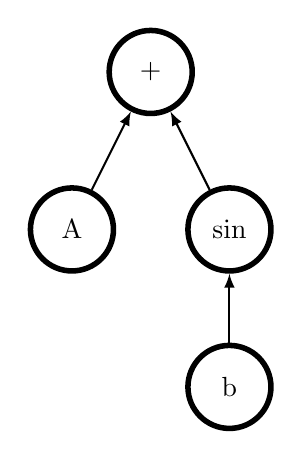
\begin{tikzpicture}[main/.style={draw, circle, minimum size=30pt, line width=2pt}, info/.style={rectangle, rounded corners=5, draw}, n/.style={-latex, line width=0.75pt}, d/.style={-latex, line width=0.75pt, dashed}]
        % nodes
        \node[main] (A) at (0,2) {\codeword{A}};
        \node[main] (b) at (2,0) {\codeword{b}};
        \node[main] (+) at (1,4) {\codeword{+}};
        \node[main] (sin) at (2,2) {\codeword{sin}};
        % edges
        \draw [->, n] (A) -- (+);
        \draw [->, n] (b) -- (sin);
        \draw [->, n] (sin) -- (+);
    \end{tikzpicture}
    \caption{Binary expression tree generated from the expression string \texttt{A + sin(b)}. Empty nodes are omitted.}
    \label{fig:tree_example}
\end{figure}

\section{Preprocessing}
Having described how a binary expression tree is created from a given tensor expression, we now describe how this tree is processed further to prepare it for differentiation.
We employ the following three preprocessing steps.
\begin{itemize}
    \item Some subtrees are substituted with equivalent ones which are more easily differentiated.
    \item Subtrees which occur more than once are fused.
    \item Each node's output tensor order is determined and stored.
\end{itemize}

\subsection{Equivalent Subtree Substitution}
Some operations or functions may be viewed as equivalent to, or as a special case of another, more easily differentiable operation or function.
In these cases, we substitute the more general case to reduce the number of differentiation rules that need to be implemented.
For example, when encountering the expression \codeword{A - B}, we substitute \codeword{A + -(B)}, viewing \codeword{-} as an elementwise function.
This allows us to use the differentiation rules for sums and elementwise functions, not having to implement a new rule for differences.
A full overview of the substituted expressions can be seen in Table \ref{tab:substitutions}.
\begin{table}[ht]
    \centering
    \begin{tabular}{l | l}
        Original & Substitute \\\hline
        \codeword{A - B} & \codeword{A + -(B)} \\
        \codeword{A ^ B} & \codeword{exp(b * log(a))} \\
        \codeword{A / B} & \codeword{A .* elementwise_inverse(B)} \\
        \codeword{adj(X)} & \codeword{det(X) *(,ij->ij) inv(X)} \\ 
    \end{tabular}
    \caption{Table showing all operations that get substituted during preprocessing, along with their substitutes. Note that \texttt{.*} is a placeholder for elementwise multiplication and \texttt{*} a placeholder for scalar multiplication. Both are replaced with the appropriate tensor products during tensor order determination. \texttt{elementwise\_inverse} is an elementwise function for which a differentiation rule is implemented.}
    \label{tab:substitutions}
\end{table}
\FloatBarrier

\subsection{Common Subtree Elimination}
When differentiating, we need to be able to tell when a subexpression is reached multiple times.
To help with this, and also to reduce the number of nodes in the expression tree, we fuse subtrees that occur more than once.

First, to identify duplicate subtrees, the notion of equality needs to be defined for trees.
We define equality of two trees, $A$ and $B$, as follows.
$$
A = B \iff \text{root}(A) = \text{root}(B) \land \text{left}(A) = \text{left}(B) \land \text{right}(A) = \text{right}(B)
$$
where $\text{root}(X)$ refers to the root node of $X$, and $\text{left}(X)$, $\text{right}(X)$ to the left and right child trees of $X$, respectively.
Equality of nodes is handled by comparing all components of the node (node type, name, indices for product nodes) individually.

Now that we may identify when two subtrees are equal, we continue with common subtree elimination.
We first obtain all subtrees by traversing the whole tree.
Then, we store each unique subtree we find in a hash table.
When we encounter a subtree that is already present in our hashmap, we let its parent node point to the tree in the hashmap instead of the original.
In doing so, we remove duplicate subtrees and transform the binary expression tree into a directed acyclic graph (DAG) representing the expression.
Nodes in the DAG still only have two child nodes, but may have many parent nodes.

\begin{figure}
    \centering
    \begin{minipage}{7cm}
        \centering
        \scalebox{0.8}{
        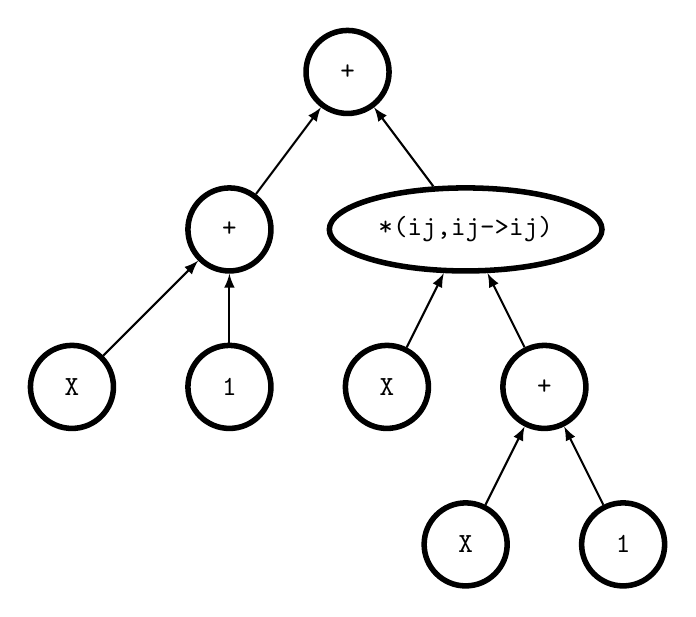
\begin{tikzpicture}[main/.style={draw, circle, minimum size=30pt, line width=2pt}, info/.style={rectangle, rounded corners=5, draw}, n/.style={-latex, line width=0.75pt}, d/.style={-latex, line width=0.75pt, dashed}]
            % nodes
            \node[main] (x1) at (1,0) {\texttt{X}};
            \node[main] (11) at (3,0) {\texttt{1}};
            \node[main] (+1) at (3,2) {\texttt{+}};
            \node[main] (+2) at (4.5,4) {\texttt{+}};
            \node[main, shape=ellipse] (*) at (6,2) {\texttt{*(ij,ij->ij)}};
            \node[main] (x2) at (5,0) {\texttt{X}};
            \node[main] (+3) at (7,0) {\texttt{+}};
            \node[main] (x3) at (6,-2) {\texttt{X}};
            \node[main] (12) at (8,-2) {\texttt{1}};
            % edges
            \draw [->, n] (x1) -- (+1);
            \draw [->, n] (11) -- (+1);
            \draw [->, n] (+1) -- (+2);
            \draw [->, n] (*) -- (+2);
            \draw [->, n] (x2) -- (*);
            \draw [->, n] (+3) -- (*);
            \draw [->, n] (x3) -- (+3);
            \draw [->, n] (12) -- (+3);
        \end{tikzpicture}}
    \end{minipage}
    \begin{minipage}{7cm}
        \centering
        \scalebox{0.8}{
        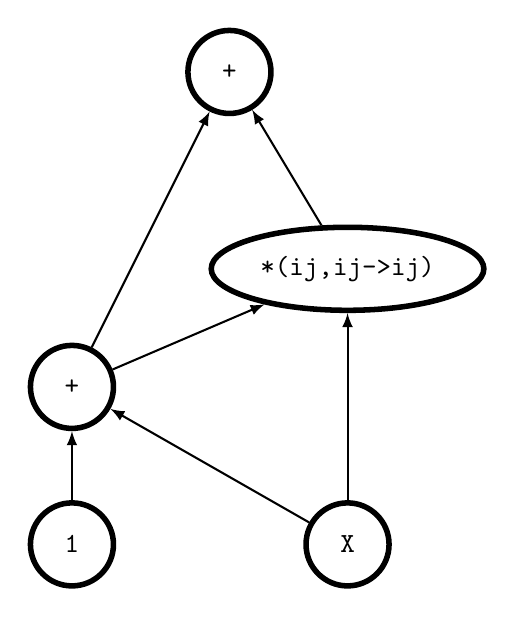
\begin{tikzpicture}[main/.style={draw, circle, minimum size=30pt, line width=2pt}, info/.style={rectangle, rounded corners=5, draw}, n/.style={-latex, line width=0.75pt}, d/.style={-latex, line width=0.75pt, dashed}]
            % nodes
            \node[main] (x1) at (3.5,0) {\texttt{X}};
            \node[main] (11) at (0,0) {\texttt{1}};
            \node[main] (+1) at (0,2) {\texttt{+}};
            \node[main] (+2) at (2,6) {\texttt{+}};
            \node[main, shape=ellipse] (*) at (3.5,3.5) {\texttt{*(ij,ij->ij)}};
            % edges
            \draw [->, n] (x1) -- (+1);
            \draw [->, n] (11) -- (+1);
            \draw [->, n] (+1) -- (+2);
            \draw [->, n] (*) -- (+2);
            \draw [->, n] (x1) -- (*);
            \draw [->, n] (+1) -- (*);
        \end{tikzpicture}}
    \end{minipage}
    \caption{Left: Binary tree generated from the expression \texttt{(X+1) + X*(ij,ij->ij) (X+1)}. Right: DAG obtained by eliminating common subtrees in the left tree.}
    \label{fig:tree_to_dag}
\end{figure}
\FloatBarrier
\subsection{Tensor order Determination}
To be able to accurately create new product nodes, which require knowledge of the tensor orders of both inputs and the output, we determine the output tensor order of all nodes in the expression DAG.
Starting at the bottom of the DAG, tensor orders are propagated upwards towards the root.
The bottom nodes contain either variables or constants.
The tensor orders of variables need to be given, as they function as the start for the upwards propagation of tensor orders.
Each parent node calculates its output tensor order based on its child nodes.
For example, a sum will have its output order set equal to the output order of its children.
A full overview of these order determination rules can be found in table \ref{tab:order_rules}.

So far we have not addressed how the tensor order of a constant is determined.
Constants may need to be broadcast to fit into the expression.
For example, in the expression \codeword{1 + det(X)} with an order 2 tensor \codeword{X}, \codeword{1} would be a scalar (order 0 tensor) since it needs to be summed with another scalar.
But in the expression \codeword{det(X + 1)}, \codeword{1} would need to be an order 2 tensor filled with ones, because it is summed with another order 2 tensor.
To accomplish this broadcasting, constants have their order set to $-1$ to start with.
Then, when an error is encountered during tensor order determination because a order $-1$ constant does not fit into a part of the expression, the order of the constant is set to the value that makes it fit.
In a sum, this would be the order of the other summand.
In a product, the order would be determined by the given input indices.
In a special function, the order is the input order the function operates on. Since all our special functions operate on matrices, this is always 2.
The case of an elementwise function is more difficult, since they operate on arbitrary input tensor orders.
Nonetheless, we may find a fitting order using the expression the output of the elementwise function is used in, by using the order that is needed there.
This is possible since the input and output order of elementwise functions are always the same.
As an example, the order of the tensor \codeword{2} in the expression \codeword{X + log(2)} may be determined by finding out what order \codeword{log(2)} needs to be to fit in the sum.
Since summands always have the same order, \codeword{log(2)}, and by extension \codeword{2}, needs to have the same order as \codeword{X}.

\begin{table}[ht]
    \centering
    \begin{tabular}{l | l}
        Parent Node Type & Output order \\\hline
        \codeword{SUM} & \codeword{order(left(X))} (= \codeword{order(right(X))}) \\
        \codeword{PRODUCT} & \codeword{output_indices(X)} \\
        \codeword{ELEMENTWISE_FUNCTION} & \codeword{order(right(X))} \\
        \codeword{adj}, \codeword{inv} & \codeword{2} \\
        \codeword{det} & \codeword{0} \\
    \end{tabular}
    \caption{Rules applied to determine tensor orders of a node \texttt{X}, depending on the type of node it is. Note that the \texttt{output\_indices} of a product node are given, and that each special function (\texttt{det}, \texttt{inv}, \texttt{adj}) needs its own rule.}
    \label{tab:order_rules}
\end{table}
\FloatBarrier

\chapter{Differentiation}
The last chapter was concerned with creating a suitable internal representation for tensor expressions, a directed acyclic graph.
In this chapter, we use this DAG representation of the expression to differentiate it.
\section{Background}
The theory for differentiating tensor expressions using our Einstein-like notation was developed by Laue, Mitterreiter and Giesen in [TENSOR PAPER].
They developed differentiation rules for DAG representations of tensor expressions based on the Fr\'{e}chet Derivative.
In their paper, they present two modes of differentiation, forward and reverse mode.
This thesis utilizes reverse mode. %TODO: Warum reverse mode statt forward mode?
In reverse mode, the computation traverses the DAG from top to bottom.
The goal is to calculate for each node $v$ the derivative of the whole expression $y$ with respect to $v$, $\frac{dy}{dv}$, also called the pullback of $v$.
Since this value is known for each parent node $u$ of $v$, we may apply the chain rule:

\begin{equation*}
    \frac{dy}{dv} = \sum_{u: (v,u) \in E} \frac{dy}{du} \cdot \frac{du}{dv}
\end{equation*}

where $(v,u) \in E$ means that there is an edge going from $v$ to $u$ in the DAG, which makes $u$ a parent of $v$. 
Note also that $\cdot$ is a placeholder for an appropriate tensor product, which is specified in the differentiation rules. 
This rule allows us to calculate the pullback of $v$ using the known pullbacks of $v$s parents $u$ and their derivatives with respect to $v$, $\frac{du}{dv}$.

This computation starts with the topmost node $y$, representing the entire expression, and computes its pullback, which is the derivative of to itself.
This pullback is then used to compute the pullback of $y$s child nodes, which are used to compute their child nodes, continuing recursively until all paths from the top node $y$ to the argument node have been traversed.
The pullback for the node containing the argument is then the result of the differentiation, the derivative of the whole expression, $y$, with respect to the argument.

\chapter{Literature}
\chapter{Appendices}
\chapter{Declaration of autonomy}

\end{document}